\section{Sprint 4}%mostrar gráficas -validaciones



\subsection{Descripción}

Uno de los aspectos más importantes desde el punto de vista del usuario es la posibilidad de generar \textit{gráficas} de manera automática con la información previamente cargada. Para llevar a cabo dicha funcionalidad se deben investigar posibles tecnologías a utilizar del lado del cliente (preferentemente basadas en \textit{javascript}, por ya conocer esta tecnología). En el caso de que la tecnología no provea soporte directo para \textit{AngularJS} se deben preparar las directivas adecuadas para su manejo. Finalmente sú implementación de manera flexible, que permita extenderlo fácilmente a todos los tipos de medición devuelto por la API.

Desde el lado del \textit{backend} se vuelve imperiosa la necesidad de validación de los atributos que componen las mediciones para garantizar la uniformidad del guardado de los mismas, y así brindar de manera satisfactoria la funcionalidad antes nombrada del \textit{frontend}.



\subsection{User Stories relacionados}
La \textbf{Tabla \ref{US-Sprint4}} indicará las características de cada user story para guiarnos en el desarrollo del sprint.

\begin{table}[h]
	\centering
	\begin{tabular}{|l|p{14cm}|}
		\hline
		\multicolumn{1}{|c|}{\textbf{ID}} &
		\multicolumn{1}{|c|}{\textbf{Enunciado de la historia}} \\          
		\hline
		\ref{infoSalud} &
		Como paciente quiero cargar mi información personal de salud referido a mediciones (altura, grasa corporal, peso, presión arterial), para que el médico cuente con más y mejor información al momento de realizar el diagnóstico. 
		
		
		\\
		\hline
		\ref{graficaParaPaciente} &
		Como paciente quiero ver gráficas que resuman mi información en particular para poder ver mis cambios a lo largo de la historia. 
		
		
		\\
		\hline
		\ref{resumenInfo} &
		Como paciente quiero obtener un resumen de mi información de salud básica para hacer uso de la misma en caso de una emergencia. 
		
		
		\\
		\hline      
		\ref{graficaParaMedico} & Como médico quiero ver gráficas que resuman la información de un paciente para poder ver sus cambios a lo largo de la historia y así apoyar la toma de decisiones y el diagnóstico.\\
		\hline
	\end{tabular}
	\caption{Listado de \textit{User Stories} relacionados.}
	\label{US-Sprint4}
\end{table}




\subsection{Planificación}

\subsubsection{Periodo de realización}

\begin{itemize}
    \item \textbf{Inicio}: 17 de agosto del 2015.
    \item \textbf{Fin}: 11 de septiembre del 2015.
\end{itemize}


\subsubsection{Sprint Backlog}
{\scriptsize
	\begin{center} %sidewaystable
		\centering
		%\begin{adjustbox}{max width=\textheight}
		\resizebox{\textwidth}{!}
		{
			\begin{tabular}{|l|l|l|p{5cm}|l|p{1cm}|}
				\hline
				\textbf{Área a cargo} &
				\textbf{Responsable} &        
				\textbf{Revisor} &        	        
				\textbf{Tarea} &
				\textbf{US} &
				\textbf{Tiempo dedicado} \\
				\hline
				
				Back-end& Franco Canizo& Michael Manganiello & Agrega a la estructura de la API paquete para validadores generales.  & US-\ref{resumenInfo} \& US-\ref{infoSalud}& 8 horas\\ \hline
				Back-end& Franco Canizo& Michael Manganiello & Creación de validadores para números enteros positivos, fecha, fecha-hora, fecha-hora previa, string con\/sin números  & US-\ref{resumenInfo} \& US-\ref{infoSalud} & 8 horas\\ \hline
				Back-end& Michael Manganiello& Franco Canizo & filtrado de mediciones en base al tipo, fuente y unidad de medición & US-\ref{resumenInfo} \& US-\ref{infoSalud}& 9 horas \\ \hline
				Back-end& Michael Manganiello& Franco Canizo & Corrección error de comparación de fechas con información de zona horaria y fechas sin esa información & US-\ref{resumenInfo} \& US-\ref{infoSalud} & 8 horas\\ \hline
				Back-end& Michael Manganiello& Franco Canizo & Simplificación del parseo de argumentos date y datetime & US-\ref{resumenInfo} \& US-\ref{infoSalud} & 5 horas \\ \hline        
				Front-end& Iván Terreno & & Capacitación en D3 & \textbf{US-17} \& \textbf{US-15} & 18 horas \\ \hline
				Front-end& Iván Terreno& Michael Manganiello & Generación de gráficas & \textbf{US-\ref{graficaParaPaciente}} \& \textbf{US-15} & 18 horas \\ \hline        
			\end{tabular}
		}
		%\end{adjustbox}
	\end{center}
}


\subsubsection{Actividades de Integración}
\begin{figure}[h!]
  \centering
  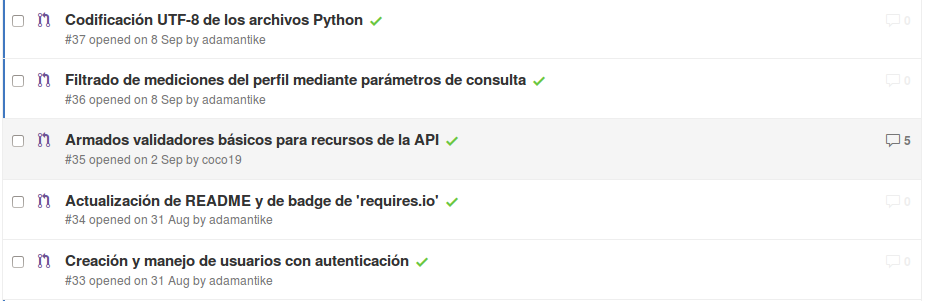
\includegraphics[width=.8\textwidth]{img/4-PR_back}
  \caption{Pull requests realizados por el back-end en el sprint 4.}
  \label{4-PR_back}
\end{figure}
\begin{figure}[h!]
  \centering
  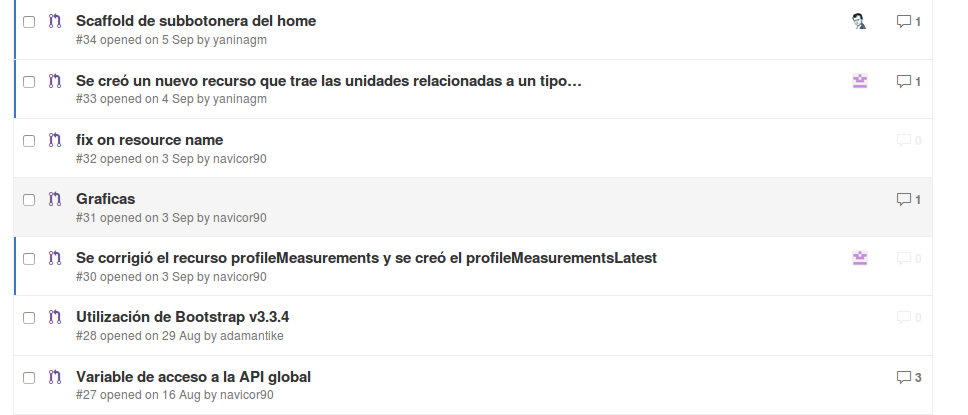
\includegraphics[width=.8\textwidth]{img/4-PR_front}
  \caption{Pull requests realizados por el front-end en el sprint 4.}
  \label{4-PR_front}
\end{figure}

	



\subsection{Modelo funcional} 


Los casos de uso de generación de gráficas y validación de datos se encuentran incluidos en las \textbf{[Figura \ref{5-cu}]} y \textbf{[\ref{5-cu-admin}]}. A continuación se realizará una breve descripción de cada caso de uso relevante involucrado:

\begin{itemize}
	\item Cargar Tipo de Medición: Permite al administrador del sistema crear un nuevo \textit{tipo de medición}, que no exista aún en el sistema. El subsistema de generación de gráficas le permite al usuario generar una gráfico en base a un \textit{tipo de medición} especificado por el usuario.
	
	\item Cargar Unidad de Medicion: Permite al administrador del sistema crear una nueva \textit{unidad de medición}, que no esté previamente cargada en el sistema. Impacta en los valores que mostrará la gráfica al consultarse.
	
	\item Mostrar Gráficas: este caso de uso se encarga de obtener las mediciones necesarias, basadas en un tipo de medición seleccionado por el usuario, y su posterior renderización para mostrarla de manera simple, visual y gráfica.
	
	\item Registrar/Editar/Eliminar Medición: es un caso de alta, baja y modificación de registros.Se debe garantizar por medio de validaciones por parte del backend la uniformidad y normalización de los datos.
	Son los datos que luego serán consultados para generar el gráfico.
	
\end{itemize}

\begin{figure}[h!]
	\centering
	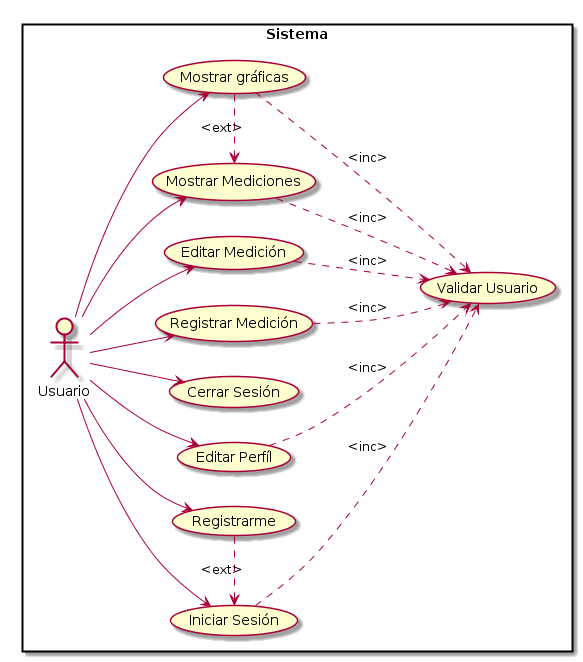
\includegraphics[width=.8\textwidth]{img/5-cu}
	\caption{Diagrama de casos de uso del sprint 4}
	\label{5-cu}
\end{figure}

\begin{figure}[h!]
	\centering
	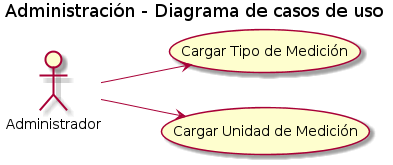
\includegraphics[width=.8\textwidth]{img/5-cu-admin}
	\caption{Diagrama de casos de uso de administración}
	\label{5-cu-admin}
\end{figure}


\subsection{Modelo de datos} 

En la \textbf{[Figura \ref{5-clases-graficas}]} podemos notar que el consumo de clases por parte de la generación de gráficas es bastante simple e inclusivo con la funcionalidad de validación de datos. Para la creación de diferentes tipos de gráficos desde una misma vista, se aprovecha la relación entre la clase \textit{Measurement} y \textit{MeasurementType} para su filtrado.

Las conexiones con la clase \textit{MeasurementUnit} nos permite mostrar al usuario el valor cargado con su unidad de medida y realizar el correspondiente filtrado en base a este parámetro.

La clase \textit{Profile} nos garantiza la obtención de las mediciones asociadas con el perfil logueado.

\begin{figure}[h!]
	\centering
	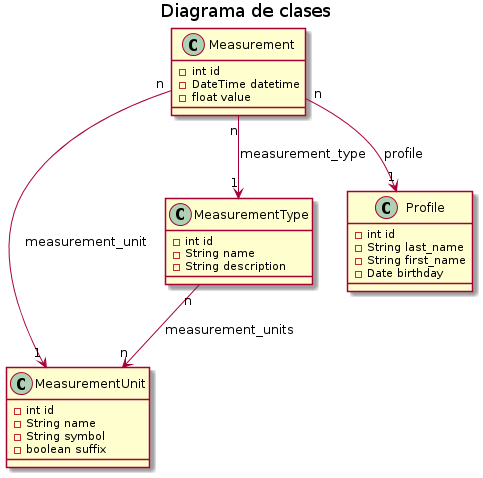
\includegraphics[width=.8\textwidth]{img/5-clases-graficas}
	\caption{Clases relevantes para el Sprint}
	\label{5-clases-graficas}
\end{figure}

A continuación se detallan las clases utilizadas y los atributos que las componen.

\subsubsection{Clase Measurement} 
Dicha clase se refiere a las medición realizada por el usuario en un momento específico. 

\textbf{Descripción de los atributos}
\begin{itemize}
	\item \textbf{id:} Identificador único de la medición (tipo int).
	\item \textbf{datetime:} Fecha y hora de la medición (tipo datetime).
	\item \textbf{value:} Valor de la medición (tipo float).
	\item \textbf{profile\_id:} Identificador único del perfil asociado (tipo int).
	\item \textbf{measurement\_source\_id:}Identificador único de la fuente de medición asociada (tipo int).
	\item \textbf{measurement\_type\_id:}Identificador único del tipo de medición asociado (tipo int).
	\item \textbf{measurement\_unit\_id:}Identificador único de la unidad de medición asociada (tipo int).
	
\end{itemize}

\subsubsection{Clase MeasurementType}
Esta clase nos permitirá  nomenclar  los tipos de medidas, hasta el momento hemos contemplado: peso, dimensión corporal (Ej:altura) y glucosa. Existen ciertas medidas que contemplan dos valores, estas serán agregadas en un sprint futuro.

\textbf{Descripción de los atributos}
\begin{itemize}
	\item \textbf{name: }	Nombre del tipo de medición(tipo string).
	\item \textbf{description:} Descripción del tipo de medición (tipo string).
\end{itemize}


\subsubsection{Clase MeasurementUnit}
Esta clase nos permitirá  nomenclar  las unidades de medición disponible para que el usuario pueda seleccionarlas cuando realice la medición, hasta el momento hemos contemplado: Kilogramo, gramo, miligramos, metro, centímetro y milímetro.

\textbf{Descripción de los atributos}
\begin{itemize}
	\item \textbf{id:	}	Identificador único de la unidad de medición(tipo int).
	\item \textbf{name :	}	Nombre de la unidad de medición ( tipo string).
	\item \textbf{symbol :}		Símbolo de la unidad de medición (tipo string).
	\item \textbf{suffix :}	Variable booleana que indica si el símbolo de la unidad de medición es un sufijo (verdadero) o un prefijo (falso) del valor de la medición (tipo boolean).
\end{itemize}



\subsection{Salidas del sistema}

El resultado de la implementación del código necesario para mostrar las gráficas del peso se puede ver en la \textbf{[Figura \ref{5-grafica_medicion}]}, aquí observamos la relación de evolución entre el día de registración de la medición y el valor asociado, en este caso para el \textit{peso}.

Debajo de la gráfica representativa de las mediciones encontramos otra miniaturizada que nos permite hacer foco en algún segmento de tiempo, para observar los valores con mayor precisión.

Además esta vista detalla de manera tabular las mediciones utilizadas para generar el gráfico.

También como resultado del sprint obtenemos algunos mensajes de error devueltos directamente por la API, por ejemplo para el caso de validación de fechas:

\begin{itemize}
	\item ``La fecha y hora ingresada no puede ser anterior al año 1900.'', para el caso en el que el usuario ingrese una fecha previa al año 1900.
	\item ``La fecha y hora ingresada no debe ser posterior a la fecha y hora actual.'', para el caso en el que el usuario ingrese una fecha posterior a la fecha y hora actual.
\end{itemize}

En la \textbf{[Figura \ref{5-msg-error}]} se puede observar el caso concreto de error devuelto ante un valor mal ingresado.

\begin{figure}[h!]
	\centering
	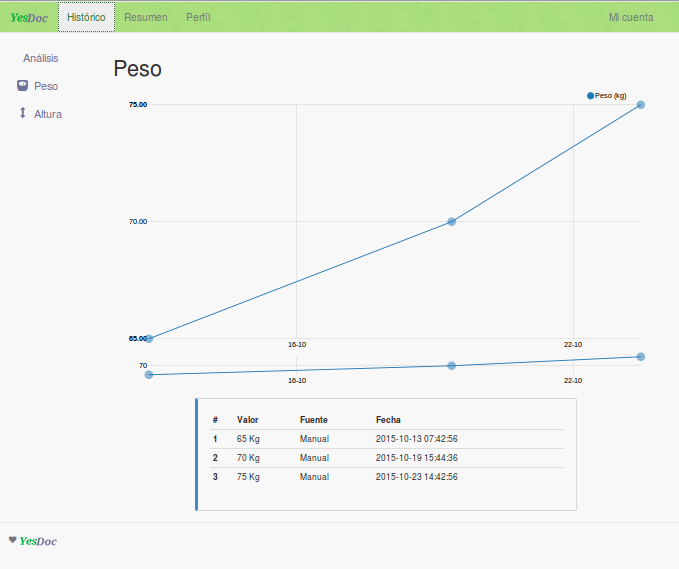
\includegraphics[width=.8\textwidth]{img/5-grafica_medicion}
	\caption{vista generada para una medición en particular}
	\label{5-grafica_medicion}
\end{figure}

\begin{figure}[h!]
	\centering
	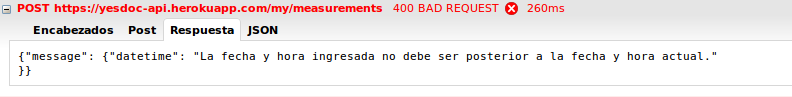
\includegraphics[width=.8\textwidth]{img/5-msg-error}
	\caption{Mensaje de error devuelto por la API}
	\label{5-msg-error}
\end{figure}

\clearpage








\subsection{Programación y documentación}

Los subsistemas de validación preparados en este sprint será útil en el desarrollo de los próximos donde intervenga la \textit{Gestión de Análisis} por la flexibilidad y desacoplamiento de sus componentes.

\subsubsection{Validadores}
El trabajo consistió en la definición de validadores usados para controlar errores y, de ser posible, sanear los datos que envían las representaciones a los recursos. Lo que se hizo es definir en un paquete una serie de validadores generales usados en el paquete \textbf{parsers} el cual se encuentra en \textbf{common}. Como podemos apreciar en la definición del parser usado por el recurso de mediciones:

\begin{lstlisting}[language=Python]
parser = reqparse.RequestParser()
parser.add_argument('datetime', type=is_valid_previous_datetime, required=True)
parser.add_argument('value', type=float, required=True)
parser.add_argument('analysis_id', type=is_valid_id, required=True)
parser.add_argument('profile_id', type=is_valid_id, required=True)
parser.add_argument('measurement_source_id', type=is_valid_id)
parser.add_argument('measurement_type_id', type=is_valid_id, required=True)
parser.add_argument('measurement_unit_id', type=is_valid_id, required=True)
\end{lstlisting}

Se define en el argumento type el llamado a una función is\_valid\_previous\_datetime, está función está definida en el paquete validators en el archivo generic validators.

\begin{lstlisting}[language=Python]
datetime_var = is_valid_datetime(var)
if datetime_var.year < 1900:
raise ValueError("La fecha y hora ingresada no puede ser anterior al anio 1900.")
elif datetime_var > datetime.utcnow():
raise ValueError("La fecha y hora ingresada no debe ser posterior a la fecha y hora actual.")
else:
return datetime_var
\end{lstlisting}

Este a su vez llama al validador is\_valid\_datetime para controlar que el dato ``datetime'' tenga un valor de fecha-hora correcto. Si el validador no encuentra error devuelve la fecha-hora, en caso contrario lanza un error.
En este parser también se define un método para controlar que el id recibido es valido, por el momento lo que hace este es controlar que el id recibido sea positivo.
\begin{comment}
Se podría poner como cosas a mejorar la validación de id.
\end{comment}




\subsubsection{Filtrado de mediciones}
El backend identifica como útil la definición de un recurso que permita devolver medidas de un perfil específico filtradas según tipo, fuente y unidad de medida. Para esto se agregó un recurso \/profile\/id\/measurements en el archivo principal de la aplicación y un recurso que define un método get para responder a una solicitud HTTP con operador GET. El mismo utiliza los datos recibidos en el ``query string'' de la URL para determinar según que tipo, fuente o unidad de medida debe filtrar. El recurso en sí no se encarga del filtrado sino que toma los datos verificados por el parse, obtiene los datos del query string y pasa estos datos a un método auxiliar definido en el archivo measurement del paquete persistence de la API ``get\_by\_profile'' el cual devuelve todas las instancias existentes de medición, asociadas a un perfil específico, ordenadas por fecha y hora de la medición, y filtradas por fuente, tipo y unidad de medición. Una vez recibida la respuesta arma el response con el código de estado correspondiente y en el cuerpo los datos resultantes serializados de acuerdo a la representación utilizada.

\begin{comment}
Faltaría agregar algunas pruebas con curl y algo de código.
Poner que se desarrollo para pasar datos específicos para que el front-end presente datos resumidos cuando estos son muchos y complejos??
\end{comment}

\subsection{Planificación de pruebas}
\subsubsection{Criterios de aceptación}
\begin{center}
	\begin{longtable}{|p{0.5cm}|p{4cm}|p{4cm}|p{5cm}|}
		\hline \hline \rowcolor[gray]{0.9}
		\multicolumn{4}{||c|}{\textbf{Criterio de aceptación}} \\
		\hline  \rowcolor[gray]{0.9}
		\textbf{Id} &
		\textbf{Contexto} &
		\textbf{Evento}&
		\textbf{Resultado} \\
		\hline
		1&En caso de que se envíe como id un valor menor o igual a 0 en cualquier representación  de una solicitud & Al ejecutar el método post, get, delete o put correspondiente del recurso & El sistema devolverá un json con el mensaje de error por entero no positivo y el código de error 400 \\ \hline
		\hline
		2&En caso de que se indique una fecha cuyo año sea menor a 1900 & al ejecutar el validador is\_valid\_previous\_date del argumento  & El sistema devolverá un json con el mensaje de error correspondiente a una fecha previa no permitida y el código de estado 400 \\ 		\hline
		\hline
		3&En caso de que se indique en la solicitud una fecha-hora con formato invalida 
		& Al ejecutar el validador \textbf{ is\_valid\_datetime}  & El sistema devolverá un json con el mensaje de error correspondiente a una fecha hora con formato inválido y el código de estado 400\\ \hline
		\hline
		4&En caso de que no exista un usuario registrado con el id indicado & al ejecutar el método get\/put del recurso \/users\/id  & El sistema devolverá un json con un mensaje de error y un código de error 404 \\ \hline
		\hline
		5&En caso de que no exista un perfil registrado con el id indicado & al ejecutar el método get del recurso \/profile\/id\/measurements  & El sistema devolverá un json con un mensaje de error por no encontrar la instancia correspondiente \\ \hline
		
	\end{longtable}
\end{center}

\begin{comment}
Cuando paso un entero no positivo no responde con error sino que query or get 404 no encuentra el registro.
El método get_latest_by_profile es del sprint2 cierto?
\end{comment}



\subsection{Retroalimentación de pruebas}
\subsubsection{Estado inicial}
A continuación se detalla la situación en la que quedaron las pruebas ejecutadas en los sprint anteriores, luego se desarrollarán las soluciones que se usaron y por última se cambiará el estado de aquellas errores encontrados por \textit{"cerrado"}.
        %
	\begin{itemize}
		\item \textbf{¿Qué fue bien?}
        	\begin{itemize}
				\item        Las cargas y muestra de mediciones en forma gráfica se llevan a cabo correctamente.
			\end{itemize}

   		\item \textbf{¿Qué se mejoró?}
        	\begin{itemize}
				\item \textbf{Cerrado} Al crear una nueva medición, se mostraba un cartel (alert de javascript) con una fecha, dicho alert fue eliminado.
                \item \textbf{Cerrado} Se encontró un problema con la zona horaria que usa el servidor y la zona horaria del usuario, para solucionarlo hubo q hacer un casteo previo cuando se solicitaba la fecha y hora del usuario para mostrar.
			\end{itemize}

   		\item \textbf{¿Qué se puede mejorar?}
        	\begin{itemize}
		        \item \textbf{Abierto} Solo debería mostrarse las unidades relacionadas al tipo de medición que se ha seleccionado 
				\item \textbf{Abierto} En el futuro se deberá mejorar las validaciones de los datos a la hora de cargar información en los formularios.
        		\item \textbf{Abierto} Se deberá mejorar la manera de seleccionar la fecha y la hora. 
                \item \textbf{Abierto} Deberá realizarse los carteles de advertencia necesarios.
            \end{itemize}
       
	\end{itemize}



\subsubsection{Estado final de pruebas}

	\begin{itemize}
		\item \textbf{¿Qué fue bien?}
        	\begin{itemize}
				\item        Las validaciones.
			\end{itemize}
            
		\item \textbf{¿Qué fue mal?}
        	\begin{itemize}
				\item        La librería que se utilizó al principio ``lvd3'' era de muy bajo nivel, por ello tuvo q cambiarse a D3 que es de más alto nivel. 
			\end{itemize}
            
   		\item \textbf{¿Qué se mejoró?}
        	\begin{itemize}
            	\item \textbf{Cerrado} Mal rendimiento de D3, mejorado usando código de la libreria lvd3
            	\item \textbf{Cerrado} Función de maximizar
                \item \textbf{Cerrado} Facilitar el pasaje del scope al controlador
                \item \textbf{Cerrado} Se encontró un problema con la zona horaria que usa el servidor y la zona horaria del usuario, para solucionarlo hubo q hacer un casteo previo cuando se solicitaba la fecha y hora del usuario para mostrar.
			\end{itemize}
       
	\end{itemize}